\documentclass[reqno]{../../../Projects/LaTeX/gtpart}

% \kern-1em % negative \quad.
% \kern-2em % negative \qquad.

\usepackage{minted}
\usepackage[scale=1.5]{strands}

\title[Strands package]{Strands package}

\author[D. Arcis]{Diego Arcis}
\address{Facultad de Ciencias de la Salud, Universidad Aut\'onoma de Chile - Sede Talca, 5 Poniente 1670, Talca 3460000, Chile.}
\email{diego.arcis@uautonoma.cl}

%\subject{primary}{msc2010}{05A18}

\numberwithin{equation}{section}

\begin{document}

\maketitle

\begin{minted}{latex}
	\usepackage[<options>]{strands}
\end{minted}

\section{The \mintinline{latex}{\vpartition} macro}

Use the macro \mintinline{latex}{\vpartition} to draw a set partition in the partition monoid $C_n$ as\[\mintinline{latex}{\vpartition[<options>]{<sorted blocks>}}\]where \mintinline{latex}{<sorted blocks>} are the blocks, separated by commas, entered as blocks of a set partition of $\{\pm1,\ldots,\pm n\}$. The positive numbers correspond to the dots above and the negative numbers correspond to the dots below. For instance:\[\begin{array}{c}
\vpartition{{1,3,-3,-4,-6},{6,5,-5,-2},{-1,2}}\\
\mintinline{latex}{\vpartition{{1,3,-3,-4,-6},{6,5,-5,-2},{-1,2}}}
\end{array}\]Note that the dots are connected in the order as the numbers appear on the blocks. So, if we change the position of numbers it will output a different representation.

The options \mintinline{latex}{<options>} are entered as \mintinline{latex}{<option>=<value>} and defined as follows:
\begin{itemize}
\item \mintinline{latex}{bend}: Integer number to manage the bend of brackets. Default value is $45$.
\item \mintinline{latex}{bulla}: Use $1$ to draw bullets from $1$ to $n$ above, otherwise use $0$. Default value is $1$.
\item \mintinline{latex}{bullb}: Use $1$ to draw bullets from $-1$ to $-n$ below, otherwise use $0$. Default value is $1$.
\item \mintinline{latex}{floor}: Nonnegative float number setting where the picture starts to be drawn. So it starts at \mintinline{latex}{floor}$*$\mintinline{latex}{height}. Default value is $0$.
\item \mintinline{latex}{font}: Nonnegative float number setting the size of the font labelling the dots. Default value is $0.7$.
\item \mintinline{latex}{height}: Positive float number setting the height of the picture. Default value is $1$. 
\item \mintinline{latex}{labelver}: Space between dots and labels. Default value is $0.2$.
\item \mintinline{latex}{labelhor}: Additional space between labels (only for signed labels). Default value is $0.03$.
\item \mintinline{latex}{norma}: Positive float number to normalize the height above \mintinline{latex}{floor} with other pictures. Default value is $0$.
\item \mintinline{latex}{normb}: Negative float number to normalize the height below \mintinline{latex}{floor} with other pictures. Default value is $0$.
\item \mintinline{latex}{nstr}: Positive integer defining the number of strands. This value is used only if it is bigger than the self computed value.
\item \mintinline{latex}{reflect}: Use $1$ to mirror the brackets connections vertically, otherwise use $0$. Default value is $0$.  
\item \mintinline{latex}{rotate}: Integer number to rotate the picture. Default value is $0$.
\item \mintinline{latex}{scale}: Positive float number to scale the picture. Default value is $1$.
\item \mintinline{latex}{strwidth}: Positive float number to set the width of the strands. Default value is $0.7$.
\item \mintinline{latex}{tkzpic}: Use $1$ to add the \mintinline{latex}{tikzpicture} environment automatically, otherwise use $0$. Default value is $1$. Note that options \mintinline{latex}{rotate} and \mintinline{latex}{scale} will not work if \mintinline{latex}{tkzpic} is $0$.
\item \mintinline{latex}{type}: Value in $\{-1,1,2,3,4,5\}$ to set the labels of the dots. Use $-1$ to put only labels below from $1$ to $n$. Use $0$ to put no labels. Use $1$ to put only labels above from $1$ to $n$. Use $2$ to put labels above and below from $1$ to $n$. Use $3$ to put labels from $1$ to $n$ above and labels from $n+1$ to $2n$ below. Use $4$ to put labels from $1$ to $n$ above and labels from $1'$ to $n'$ below. Use $5$ to put signed labels, $n$ must be even in this case.
\item \mintinline{latex}{width}: Positive float number to set the width between horizontal dots. Default value is $0.6$.
\end{itemize}
Most of the options defined above can be set as global options in the \mintinline{latex}{\usepackage} macro.

Below a more complex example:\[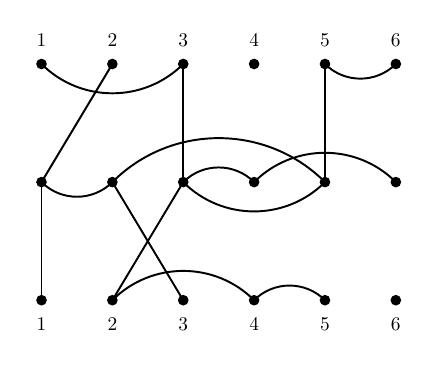
\begin{tikzpicture}[scale=1.5]
\vpartition[
	bullb=0,
	floor=1,
	tkzpic=0,
	type=1
]{{1,3,-3,-4,-6},{6,5,-5,-2},{-1,2}}
\vpartition[
	nstr=6,
	tkzpic=0,
	type=-1
]{{-1,1,2,-3},{5,3,-2,-4,-5}}
\end{tikzpicture}\]

\begin{minted}{latex}
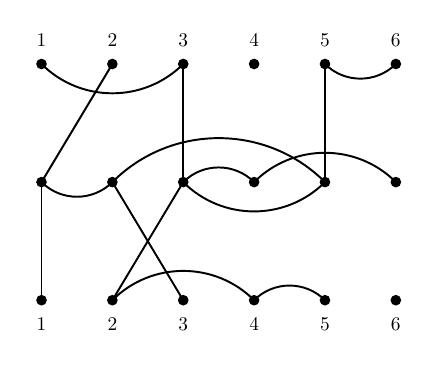
\begin{tikzpicture}[scale=1.5]
	\vpartition[
		bullb=0,
		floor=1,
		tkzpic=0,
		type=1
	]{{1,3,-3,-4,-6},{6,5,-5,-2},{-1,2}}
	\vpartition[
		nstr=6,
		tkzpic=0,
		type=-1
	]{{-1,1,2,-3},{5,3,-2,-4,-5}}
\end{tikzpicture}
\end{minted}

\subsection{The \mintinline{latex}{\arcpartition} macro}

Use the macro \mintinline{latex}{\arcpartition} to draw the graph of a set partition of $\{1,\ldots,n\}$ as\[\mintinline{latex}{\arcpartition[<options>]{<sorted blocks>}}\]where \mintinline{latex}{<sorted blocks>} are the blocks, separated by commas. This macro is constructed from \mintinline{latex}{\vpartition}, so its behavior is similar. For instance:\[\begin{array}{c}
\arcpartition{{1,4},{2,3,7}}\\
\mintinline{latex}{\arcpartition{{1,4},{2,3,7}}}
\end{array}\]

The options \mintinline{latex}{<options>} come from \mintinline{latex}{\vpartition}, so most of them are defined in the same way, these are: \mintinline{latex}{bend}, \mintinline{latex}{floor}, \mintinline{latex}{font}, \mintinline{latex}{labelver}, \mintinline{latex}{lavelhor}, \mintinline{latex}{norma}, \mintinline{latex}{normb}, \mintinline{latex}{rotate}, \mintinline{latex}{scale}, \mintinline{latex}{strwidth}, \mintinline{latex}{tkzpic} and \mintinline{latex}{width}. However, the following options work different:

\begin{itemize}
\item \mintinline{latex}{bull}: Use $1$ to draw bullets from $1$ to $n$. Otherwise use $0$. Default value is $1$.
\item \mintinline{latex}{num}: Positive integer defining the number of dots. This value is used only if it is bigger than the self computed value.
\item \mintinline{latex}{type}: Use $1$ to put labels from $1$ to $n$, otherwise use $0$. Default value is $1$.
\end{itemize}
Most of the options can be set as global options in the \mintinline{latex}{\usepackage} macro.

\section{The \mintinline{latex}{\strands} macro}

\subsubsection*{Acknowledgements}
The author was supported by the grant "Fondo de Apoyo a la Investigaci\'on" DIUA179-2020.

\bibliographystyle{plainurl}
\bibliography{../../../Projects/LaTeX/bibtex}

\end{document}